\tikzset{every picture/.style={line width=0.75pt}}

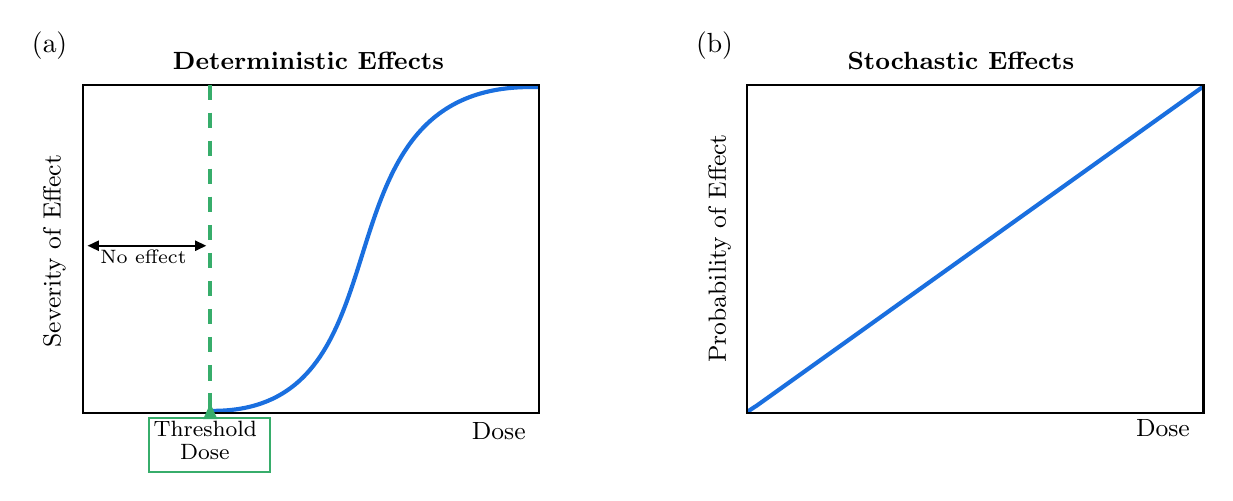
\begin{tikzpicture}[x=0.75pt,y=0.75pt,yscale=-1,xscale=1]

%Straight Lines [id:da7730700763729692] 
\draw [color={rgb, 255:red, 26; green, 111; blue, 223}  ,draw opacity=1 ][line width=1.5]    (599.76,48.96) -- (385.01,202.42) -- (380.42,205.43) ;
%Curve Lines [id:da8629624283311327] 
\draw [color={rgb, 255:red, 26; green, 111; blue, 223}  ,draw opacity=1 ][line width=1.5]    (121.47,205.11) .. controls (198.34,206.12) and (184.08,114.95) .. (221.47,71.53) .. controls (233.7,57.34) and (251.44,48.25) .. (279.69,49.16) ;
%Shape: Rectangle [id:dp07258514804006644] 
\draw  [line width=0.75]  (60,48) -- (280,48) -- (280,206) -- (60,206) -- cycle ;
%Straight Lines [id:da09166760913517435] 
\draw [color={rgb, 255:red, 55; green, 173; blue, 107}  ,draw opacity=1 ][line width=1.5]  [dash pattern={on 5.63pt off 4.5pt}]  (121.38,47.92) -- (121.38,206.32) ;
%Straight Lines [id:da3468358858445303] 
\draw    (65.4,125.56) -- (116.52,125.56) ;
\draw [shift={(119.52,125.56)}, rotate = 180] [fill={rgb, 255:red, 0; green, 0; blue, 0 }  ][line width=0.08]  [draw opacity=0] (5.36,-2.57) -- (0,0) -- (5.36,2.57) -- cycle    ;
\draw [shift={(62.4,125.56)}, rotate = 0] [fill={rgb, 255:red, 0; green, 0; blue, 0 }  ][line width=0.08]  [draw opacity=0] (5.36,-2.57) -- (0,0) -- (5.36,2.57) -- cycle    ;
%Shape: Rectangle [id:dp4467912586395093] 
\draw  [color={rgb, 255:red, 55; green, 173; blue, 107}  ,draw opacity=1 ] (91.8,208.57) -- (150.3,208.57) -- (150.3,234.63) -- (91.8,234.63) -- cycle ;
%Shape: Triangle [id:dp7577642747879886] 
\draw  [color={rgb, 255:red, 55; green, 173; blue, 107}  ,draw opacity=1 ][fill={rgb, 255:red, 55; green, 173; blue, 107}  ,fill opacity=1 ] (121.5,202.71) -- (124.14,208.56) -- (118.85,208.56) -- cycle ;
%Shape: Rectangle [id:dp10920079476550804] 
\draw  [line width=0.75]  (380,48) -- (600,48) -- (600,206) -- (380,206) -- cycle ;

% Text Node
\draw (102,31) node [anchor=north west][inner sep=0.75pt]  [font=\small] [align=left] {\textbf{Deterministic Effects}};
% Text Node
\draw (67,126) node [anchor=north west][inner sep=0.75pt]  [font=\small] [align=left] {{\scriptsize No effect}};
% Text Node
\draw (427,31) node [anchor=north west][inner sep=0.75pt]  [font=\small] [align=left] {\textbf{Stochastic Effects}};
% Text Node
\draw (246,209) node [anchor=north west][inner sep=0.75pt]  [font=\small] [align=left] {Dose};
% Text Node
\draw (566,208) node [anchor=north west][inner sep=0.75pt]  [font=\small] [align=left] {Dose};
% Text Node
\draw (39.5,176) node [anchor=north west][inner sep=0.75pt]  [font=\small,rotate=-270] [align=left] {Severity of Effect};
% Text Node
\draw (360,183.33) node [anchor=north west][inner sep=0.75pt]  [font=\small,rotate=-270] [align=left] {Probability of Effect};
% Text Node
\draw (92.7,208.5) node [anchor=north west][inner sep=0.75pt]  [font=\small] [align=left] {{\footnotesize Threshold}};
% Text Node
\draw (105.45,219.83) node [anchor=north west][inner sep=0.75pt]  [font=\small] [align=left] {{\footnotesize Dose}};
% Text Node
\draw (34,21) node [anchor=north west][inner sep=0.75pt]   [align=left] {(a)};
% Text Node
\draw (354,21) node [anchor=north west][inner sep=0.75pt]   [align=left] {(b)};
\end{tikzpicture}
